\documentclass{article}

\usepackage{amsmath,amssymb}
\usepackage{tikz}
\usepackage{pgfplots}
\usepackage{xcolor}
\usepackage[left=2.1cm,right=3.1cm,bottom=3cm,footskip=0.75cm,headsep=0.5cm]{geometry}
\usepackage{enumerate}
\usepackage{enumitem}
\usepackage{marvosym}
\usepackage{tabularx}
\usepackage{parskip}
\usepackage{longtable}

\usepackage{listings}
\definecolor{lightlightgray}{rgb}{0.95,0.95,0.95}
\definecolor{lila}{rgb}{0.8,0,0.8}
\definecolor{mygray}{rgb}{0.5,0.5,0.5}
\definecolor{mygreen}{rgb}{0,0.8,0.26}
%\lstdefinestyle{java} {language=java}
\lstset{language=R,
	basicstyle=\ttfamily,
	keywordstyle=\color{lila},
	commentstyle=\color{lightgray},
	stringstyle=\color{mygreen}\ttfamily,
	backgroundcolor=\color{white},
	showstringspaces=false,
	numbers=left,
	numbersep=10pt,
	numberstyle=\color{mygray}\ttfamily,
	identifierstyle=\color{blue},
	xleftmargin=.1\textwidth, 
	%xrightmargin=.1\textwidth,
	escapechar=§,
	%literate={\t}{{\ }}1
	breaklines=true,
	postbreak=\mbox{\space}
}

\usepackage[colorlinks = true, linkcolor = blue, urlcolor  = blue, citecolor = blue, anchorcolor = blue]{hyperref}
\usepackage[utf8]{inputenc}

\renewcommand*{\arraystretch}{1.4}

\newcolumntype{L}[1]{>{\raggedright\arraybackslash}m{#1}}
\newcolumntype{R}[1]{>{\raggedleft\arraybackslash}m{#1}}
\newcolumntype{C}[1]{>{\centering\let\newline\\\arraybackslash\hspace{0pt}}m{#1}}

\newcommand{\E}{\mathbb{E}}
\DeclareMathOperator{\rk}{rk}
\DeclareMathOperator{\Var}{Var}
\DeclareMathOperator{\Cov}{Cov}

\title{\textbf{Finanzderivate und Optionen, Optionsstrategien}}
\author{\textsc{Henry Haustein}}
\date{}

\begin{document}
	\maketitle
	
	\begin{longtable}[t]{L{2cm}|L{3cm}|L{5cm}|l}
		\textbf{Name} & \textbf{Legs} & \textbf{Kennzahlen} & \textbf{Plot} \\
		\hline
		Bull Call Spread & $C^+<C^-$ & Max Loss: $P_{gez}$,\newline Max Profit: $E_2-E_1-P_{gez}$,\newline BEP: $E_1+P_{gez}$ & \raisebox{-.5\height}{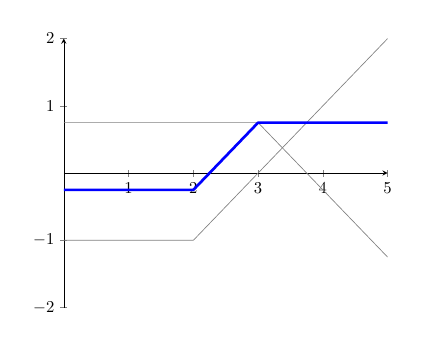
\begin{tikzpicture}[scale=0.6]
			\begin{axis}[
				xmin=0, xmax=5,
				ymin=-2, ymax=2,
				samples=400,
				axis x line=middle,
				axis y line=middle,
				domain=0:5,
				]
				\addplot[gray, no marks] {max(x-2,0)-1};
				\addplot[gray, no marks] {-max(x-3,0)+0.75};
				\addplot[blue, no marks,ultra thick] {-max(x-3,0)+0.75 + max(x-2,0)-1};
				
			\end{axis}
		\end{tikzpicture}} \\
		\hline
		Bear Call Spread & $C^-<C^+$ & Max Loss: $E_2-E_1-P_{er}$,\newline Max Profit: $P_{er}$,\newline BEP: $E_1+P_{er}$ & \raisebox{-.5\height}{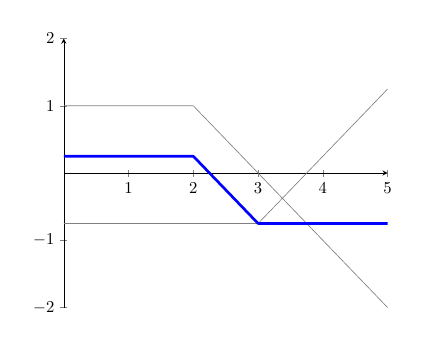
\begin{tikzpicture}[scale=0.6]
				\begin{axis}[
					xmin=0, xmax=5,
					ymin=-2, ymax=2,
					samples=400,
					axis x line=middle,
					axis y line=middle,
					domain=0:5,
					]
					\addplot[gray, no marks] {-max(x-2,0)+1};
					\addplot[gray, no marks] {max(x-3,0)-0.75};
					\addplot[blue, no marks,ultra thick] {max(x-3,0)-0.75 + -max(x-2,0)+1};
					
				\end{axis}
		\end{tikzpicture}} \\
		\hline
		Bull Put Spread & $P^+ < P^-$ & Max Loss: $E_2-E_1-P_{er}$,\newline Max Profit: $P_{er}$,\newline BEP: $E_2-P_{er}$ & \raisebox{-.5\height}{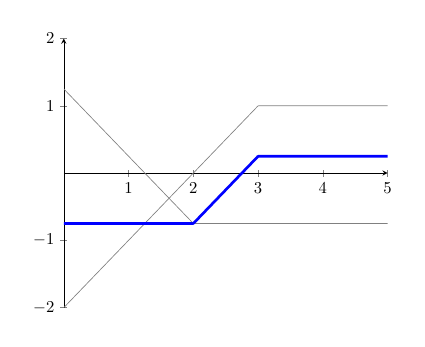
\begin{tikzpicture}[scale=0.6]
				\begin{axis}[
					xmin=0, xmax=5,
					ymin=-2, ymax=2,
					samples=400,
					axis x line=middle,
					axis y line=middle,
					domain=0:5,
					]
					\addplot[gray, no marks] {max(2-x,0)-0.75};
					\addplot[gray, no marks] {-max(3-x,0)+1};
					\addplot[blue, no marks,ultra thick] {max(2-x,0)-0.75 + -max(3-x,0)+1};
					
				\end{axis}
		\end{tikzpicture}} \\
		\hline
		Bear Put Spread & $P^- < P^+$ & Max Loss: $P_{gez}$,\newline Max Profit: $E_2-E_1-P_{gez}$,\newline BEP: $E_2-P_{gez}$ & \raisebox{-.5\height}{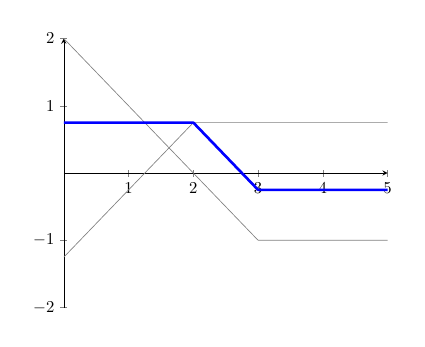
\begin{tikzpicture}[scale=0.6]
				\begin{axis}[
					xmin=0, xmax=5,
					ymin=-2, ymax=2,
					samples=400,
					axis x line=middle,
					axis y line=middle,
					domain=0:5,
					]
					\addplot[gray, no marks] {max(3-x,0)-1};
					\addplot[gray, no marks] {-max(2-x,0)+0.75};
					\addplot[blue, no marks,ultra thick] {max(3-x,0)-1 + -max(2-x,0)+0.75};
					
				\end{axis}
		\end{tikzpicture}} \\
		\hline
		Straddle & $C^+=P^+$ & Max Loss: $P_{gez}$,\newline Max Profit: $\infty$,\newline BEP: $E\pm P_{gez}$ & \raisebox{-.5\height}{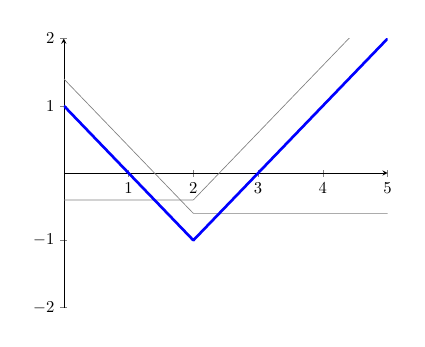
\begin{tikzpicture}[scale=0.6]
				\begin{axis}[
					xmin=0, xmax=5,
					ymin=-2, ymax=2,
					samples=400,
					axis x line=middle,
					axis y line=middle,
					domain=0:5,
					]
					\addplot[gray, no marks] {max(x-2,0)-0.4};
					\addplot[gray, no marks] {max(2-x,0)-0.6};
					\addplot[blue, no marks,ultra thick] {max(x-2,0)-0.4 + max(2-x,0)-0.6};
					
				\end{axis}
		\end{tikzpicture}} \\
		\hline
		Strangle & $C^+\neq P^+$ & Max Loss: $P_{gez}$,\newline Max Profit: $\infty$,\newline BEP: $E_1-P_{gez}$, $E_2+P_{gez}$ & \raisebox{-.5\height}{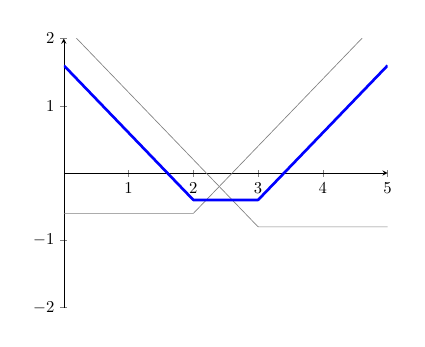
\begin{tikzpicture}[scale=0.6]
				\begin{axis}[
					xmin=0, xmax=5,
					ymin=-2, ymax=2,
					samples=400,
					axis x line=middle,
					axis y line=middle,
					domain=0:5,
					]
					\addplot[gray, no marks] {max(x-2,0)-0.6};
					\addplot[gray, no marks] {max(3-x,0)-0.8};
					\addplot[blue, no marks,ultra thick] {max(x-2,0)-0.6 + max(3-x,0)-0.8};
					
				\end{axis}
		\end{tikzpicture}} \\
		\hline
		Time Spread & Kauf längere Option, Verkauf kürzerer Option & Max Loss: $P_{gez}$,\newline Max Profit: nicht feststellbar,\newline BEP: nicht feststellbar & \\
		\hline
		Butterfly (Calls) & $C^+<2C^-<C^+$ & Max Loss: $P_{gez}$,\newline Max Profit: $E_2-E_1-P_{gez}$,\newline BEP: $E_1+P_{gez}$, $E_3-P_{gez}$ & \raisebox{-.5\height}{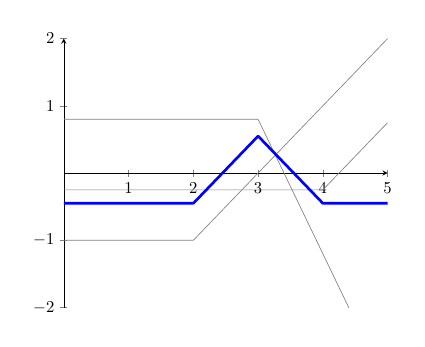
\begin{tikzpicture}[scale=0.6]
				\begin{axis}[
					xmin=0, xmax=5,
					ymin=-2, ymax=2,
					samples=400,
					axis x line=middle,
					axis y line=middle,
					domain=0:5,
					]
					\addplot[gray, no marks] {max(x-2,0)-1};
					\addplot[gray, no marks] {max(x-4,0)-0.25};
					\addplot[gray, no marks] {2*(-max(x-3,0)+0.4)};
					\addplot[blue, no marks,ultra thick] {max(x-2,0)-1 + max(x-4,0)-0.25 + 2*(-max(x-3,0)+0.4)};
					
				\end{axis}
		\end{tikzpicture}} \\
		\hline
		Butterfly (Puts) & $P^+<2P^-<P^+$ & Max Loss: $P_{gez}$,\newline Max Profit: $E_2-E_1-P_{gez}$,\newline BEP: $E_1+P_{gez}$, $E_3-P_{gez}$ & \raisebox{-.5\height}{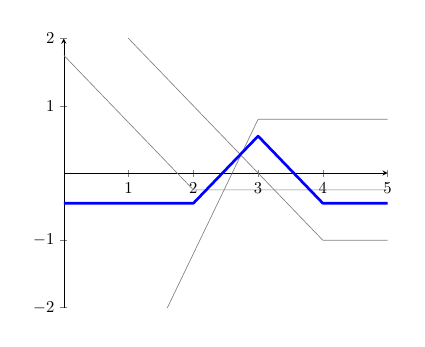
\begin{tikzpicture}[scale=0.6]
				\begin{axis}[
					xmin=0, xmax=5,
					ymin=-2, ymax=2,
					samples=400,
					axis x line=middle,
					axis y line=middle,
					domain=0:5,
					]
					\addplot[gray, no marks] {max(2-x,0)-0.25};
					\addplot[gray, no marks] {max(4-x,0)-1};
					\addplot[gray, no marks] {2*(-max(3-x,0)+0.4)};
					\addplot[blue, no marks,ultra thick] {max(2-x,0)-0.25 + max(4-x,0)-1 + 2*(-max(3-x,0)+0.4)};
					
				\end{axis}
		\end{tikzpicture}} \\
		\hline
		Box & $(C^+=P^-) < (C^-=P^+)$ & Wert einer Box (Aktienindex): $\frac{E_2-E_1}{1+\frac{r}{n}}$ \newline Wert einer Box (FI-Futures): $E_2-E_1$ & \raisebox{-.5\height}{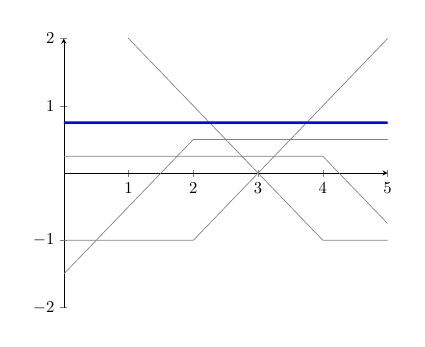
\begin{tikzpicture}[scale=0.6]
				\begin{axis}[
					xmin=0, xmax=5,
					ymin=-2, ymax=2,
					samples=400,
					axis x line=middle,
					axis y line=middle,
					domain=0:5,
					]
					\addplot[gray, no marks] {max(x-2,0)-1};
					\addplot[gray, no marks] {-max(2-x,0)+0.5};
					\addplot[gray, no marks] {-max(x-4,0)+0.25};
					\addplot[gray, no marks] {max(4-x,0)-1};
					\addplot[blue, no marks,ultra thick] {max(x-2,0)-1 + -max(2-x,0)+0.5 + -max(x-4,0)+0.25 + max(4-x,0)-1};
					
				\end{axis}
		\end{tikzpicture}}
	\end{longtable}
	
\end{document}